\documentclass[tikz]{standalone}
\usepackage[utf8]{inputenc}
\usepackage{amsmath}

\usetikzlibrary{calc}
\usetikzlibrary{backgrounds}
\def\hash{\mathrm{H}}

\begin{document}

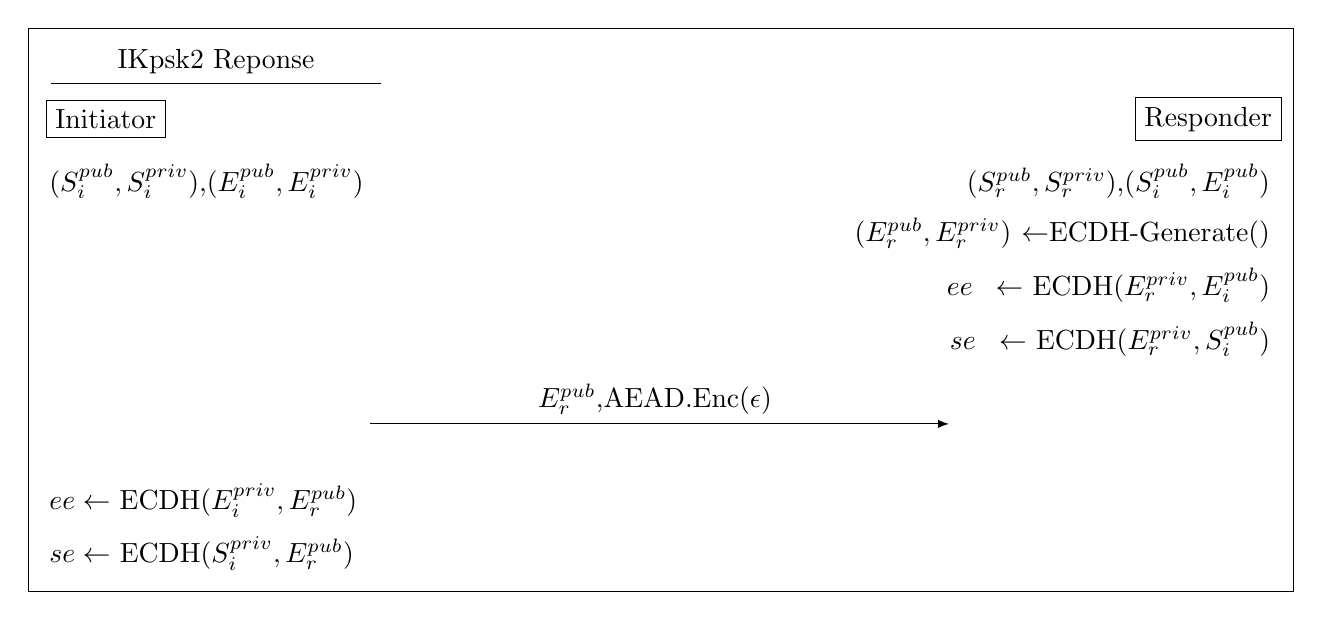
\begin{tikzpicture}[yscale=.9,xscale=.7,framed]
\tikzstyle{box}=[draw,fill=white, rectangle, rounded corners=3pt, align=left, minimum width=5.7cm, minimum height=.8cm]
  

 \draw [-] (-11, 0.5) edge node[above, align=left] {IKpsk2 Reponse} (-5,0.5);

\node (client) at (-10,0)  [draw] {Initiator}; 
\coordinate (C) at (-11.2,-0.5);
\coordinate (S) at (11.3,-0.5);

\node (StaticC) [below right,align=left,text width = 10cm] at (C.south){($S_i^{pub}, S_i^{priv}$),($E_i^{pub},E_i^{priv}$)};
%\node(kA)[below,text width = 10cm] at (StaticC.south) { Knows: $S_r^{pub}$};

\coordinate (InitEnd) at ($(C.south) + (0, -4)$);
\coordinate (InitSEnd) at ($(S.south) + (0, -4)$);

\node (server) at (10,0) [draw]{Responder};

\node(StaticS) [below left,align=right,text width =5.5cm] at (S.south) {($S_r^{pub}, S_r^{priv}$),($S_i^{pub},E_i^{pub}$)};
\node (initCkg) [below ,align=right,text width =5.5cm] at (StaticS.south) {($E_r^{pub}, E_r^{priv}) \gets $ECDH-Generate()};
\node (eer) [below ,align=right,text width = 5.5cm] at (initCkg.south) {$ee \gets$ ECDH($E_r^{priv},E_i^{pub})$};
\node (ser) [below ,align=right,text width = 5.5cm] at (eer.south) {$se \gets$ ECDH($E_r^{priv},S_i^{pub})$};

\draw[-latex,align=center] ($(InitEnd.south)+(6,0.2) $) -- ($(InitSEnd.south)+(-6,0.2)$) node [pos=0.5, above](handshake1) {$E_r^{pub}$,AEAD.Enc($\epsilon$) };


\node[below right , align=left,text width = 10cm] (eei) at ($(InitEnd.south)+(0,-0.5)$)  {$ee \gets$ ECDH($ E_i^{priv},E_r^{pub})$};
\node[below , align=left,text width = 10cm] (sei) at (eei.south)   {$se \gets$ ECDH($S_i^{priv},E_r^{pub})$};





\end{tikzpicture}

\end{document}